\chapter{T-Cell Receptor Sequence Numbering}
\label{chapterlabel1}
A robust sequence numbering method for T-cell receptors is important for all work with T-cell receptor sequence data. Universal numbering schemes and correct residue numbering is vital for sequence analysis and comparison. We present a numbering software for T-cell receptor sequences that will reliably implement a set of popular numbering schemes. The software also enables T-cell receptor sequences to be labeled using numbering schemes commonly used for antibodies, which will facilitate studying the differences and commonalities of T-cell receptors and antibodies. It will also enable antibody-based tools to be adapted to T-cell receptor sequences. The numbering software is to be made available at \url{http://www.bioinf.org.uk/abs/qualiloop/TCRnum}


Reliable sequence numbering is vital for sequence analysis and comparison. Given the lack of a universally agreed upon numbering scheme to be implemented for T-cell receptor sequences, sequence comparisons can be non-trivial. 
If TCR sequences can also be correctly numbered using schemes commonly implemented for antibody sequences, this will facilitate further research into the likeness of antibody and TCR-characteristics. 
In a paper comparing antibody and TCR CDRs,\cite{Wong2019} it was found that TCR and antibody CDRs occupy distinct areas of structural space. Understanding more about how the two relate may lead to a greater understanding of TCR and their functionality. 
The most commonly used antibody numbering schemes are arguably Kabat-, and Chothia-numbering. Therefore, numbering TCRs using these systems would be of great value for comparing TCR and antibody sequences. IMGT and Aho numbering, as two additional popular numbering schemes,will also be prove useful. 
Furthermore, having correctly numbered TCRs using the same numbering schemes commonly used for antibody sequences will facilitate the re-writing of antibody-geared tools created by Prof. Martin for TCRs. 
There are not many publicly available options available for TCR sequence numbering. An example of already existing software is ANARCI\cite{Dunbar2016}, which is a numbering tool that handles antibody as well as TCR sequences of human or murine origin. TCR sequences may be numbered according to Aho or IMGT schemes.  Furthermore, an unpublished numbering tool can be found on the tcrdb server\cite{Chen2021}, which offers a choice of Kabat or Aho numbering. However, the methods and accuracy of this tool are not publicly available. Therefore, the generation of reliable, robust numbering software that can utilize the Kabat, Chothia, IMGT and Aho scheme, would be very useful for future projects involving TCR sequences. This is especially true, when one considers the fact that all further sequence analyses is subject to correct numbering.

\section{Results}

Firstly, a web interface was created to interactively display different numbering schemes interactively. The different numbering schemes can be selected, as well as the chain type. Insertion/deletion sites according to the selected numbering scheme are denoted, as well as the CDR locations based on Kabat definitions transferred to the TCR context \ref{fig:schemes}. 
\begin{figure}
    \centering
    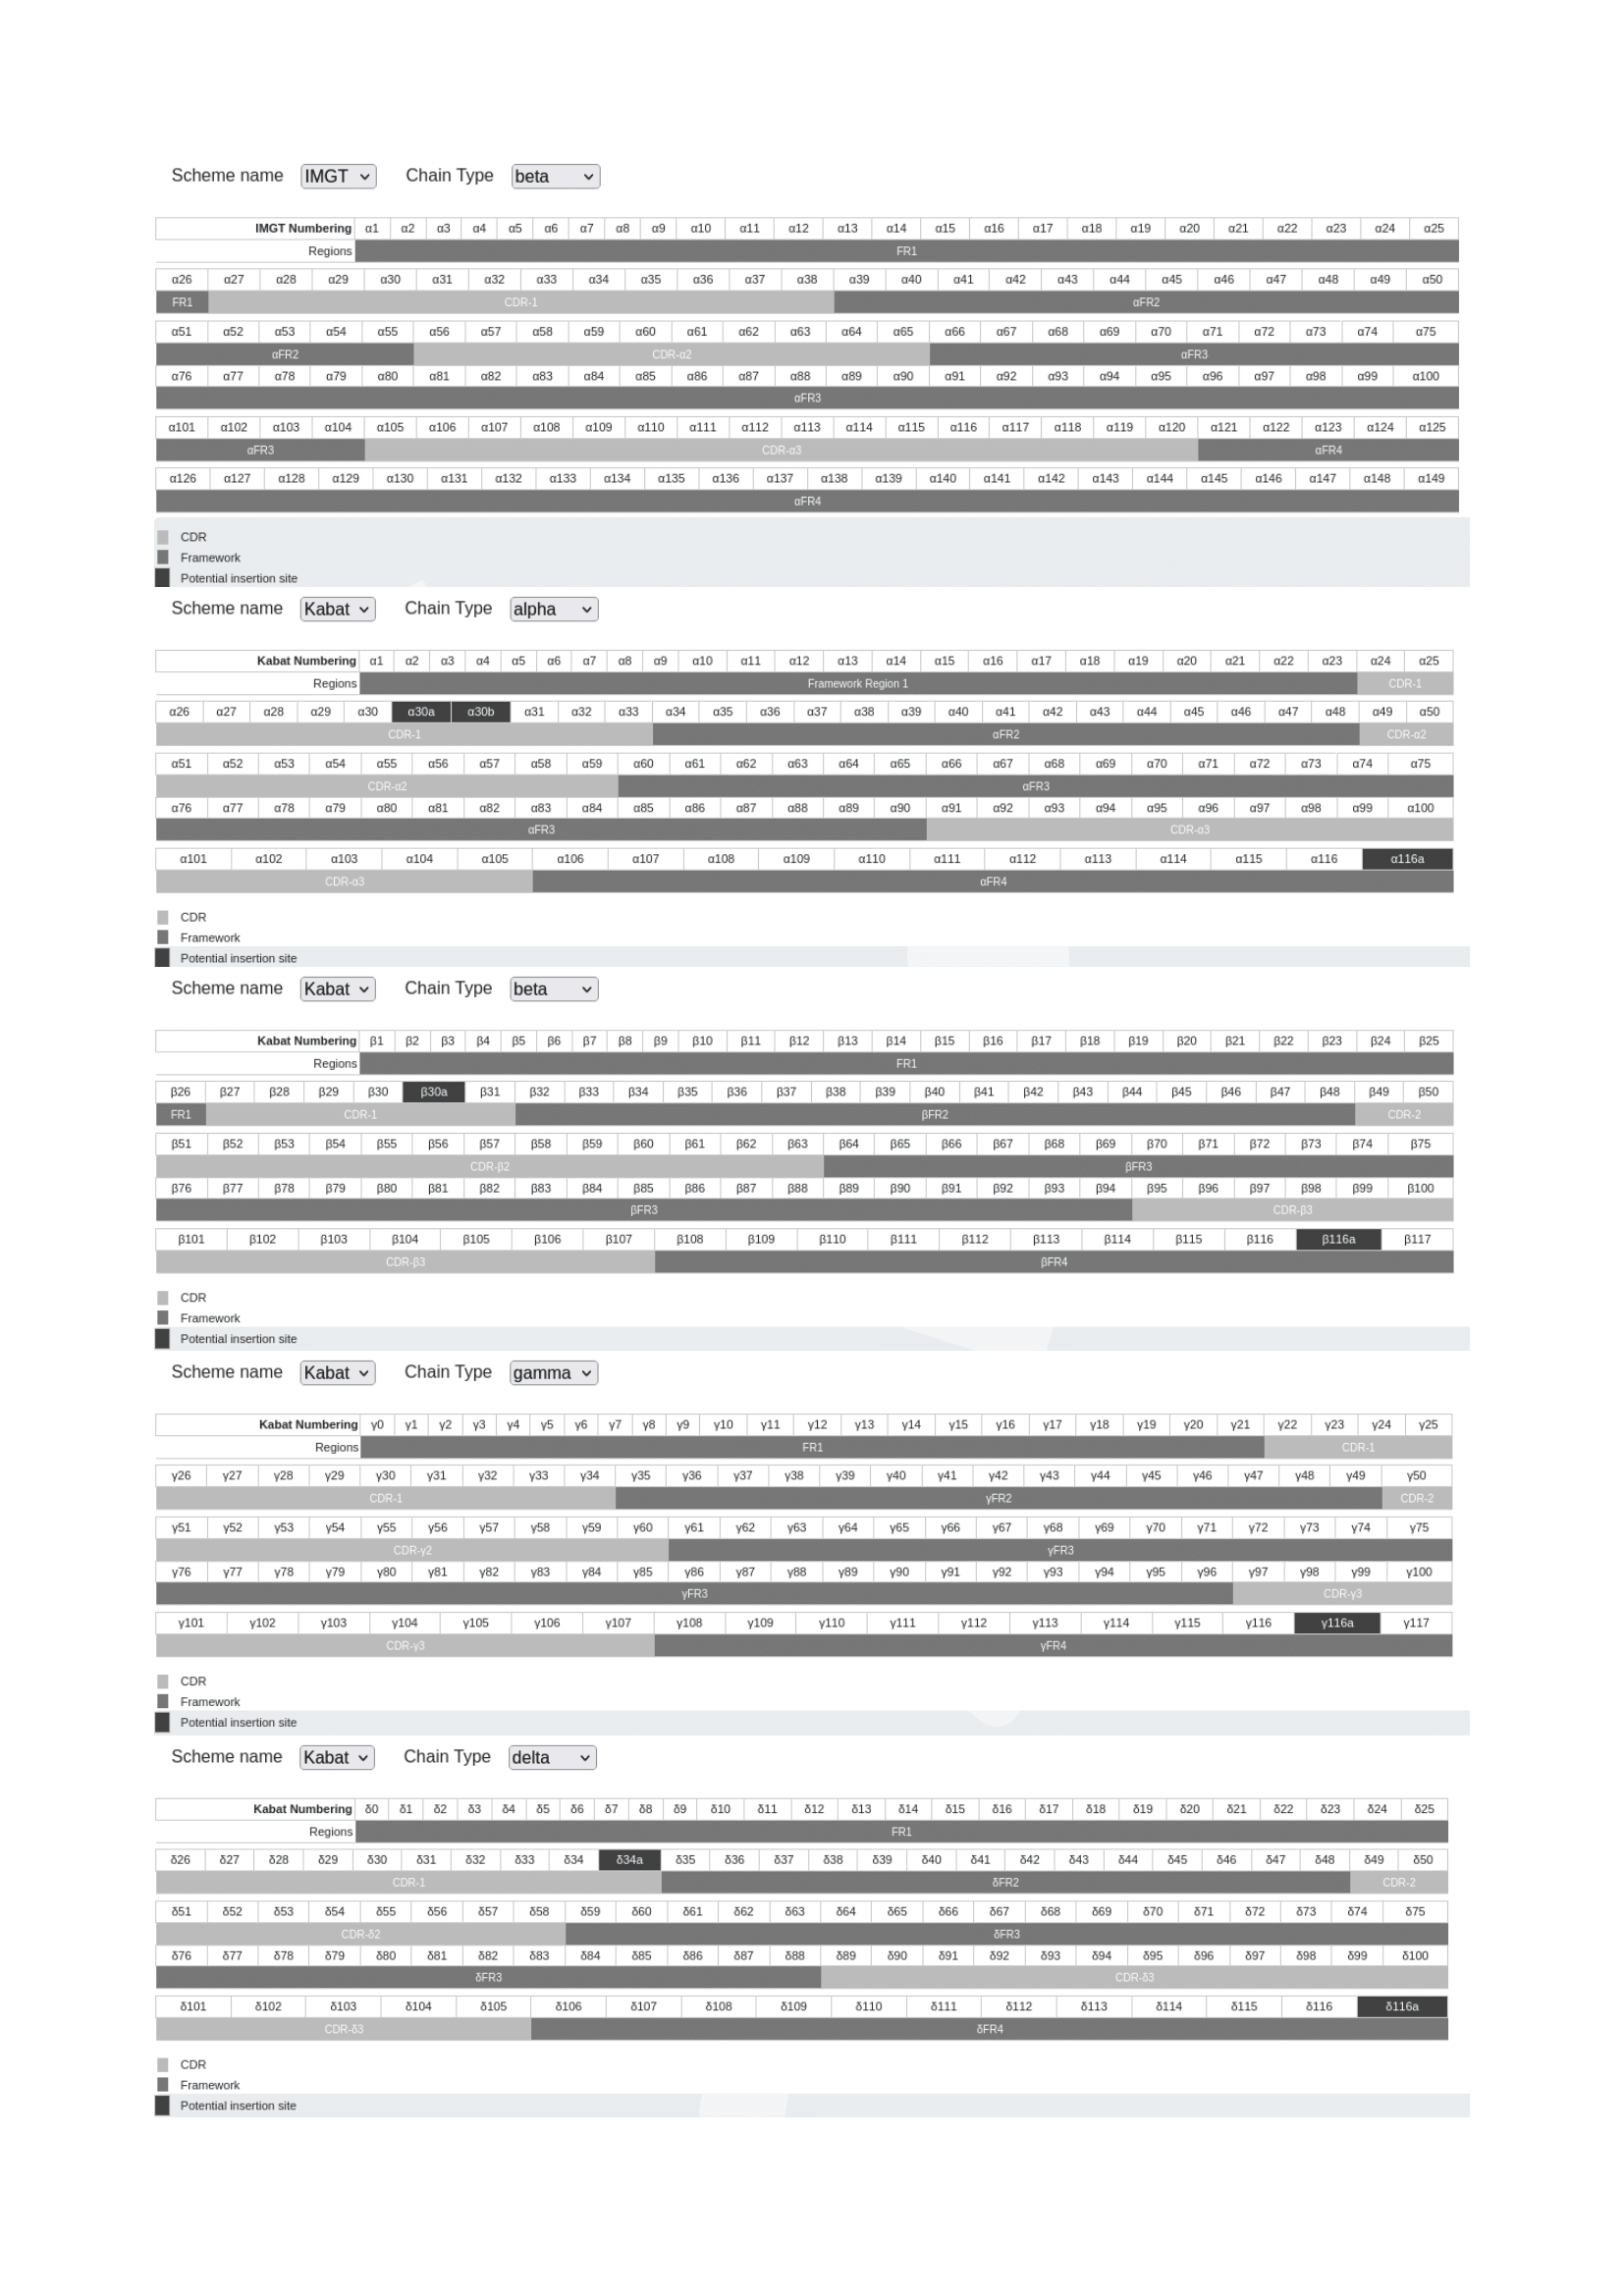
\includegraphics[width=\textwidth,height=\textheight,keepaspectratio]{schemes-1.png}
    \caption{The different numbering schemes for TCR sequences. The placement of insertions/deletions and position of the complementarity determining regions implied by the numbering scheme are displayed. (Not all numbering schemes are displayed here. For the complete set visit \url{http://www.bioinf.org.uk/abs/qualiloop/TCRnum} }
    \label{fig:schemes}
\end{figure}

In order to obtain a reliable numbering programme, a set of correctly numbered sequences for each of the numbering schemes is needed. These sequences are sorted by chain type and organism and are stored in MongoDB database collections along with the correct numbering \ref{fig:database_creation} Once the database is set up, the CDR regions within the different numbering schemes are defined. As no official Kabat or Chothia definitions of the CDR regions exist, these were arrived at using an alignment with the equivalent antibody numbering scheme\cite{AAAAA}.
Furthermore, by analysing the sequences in the newly produced mongo database, a Kabat-style definition for the TCR can be proposed \ref{fig:Aho_logo}, \ref{fig:IMGT_logo}.

\begin{figure}
    \centering
    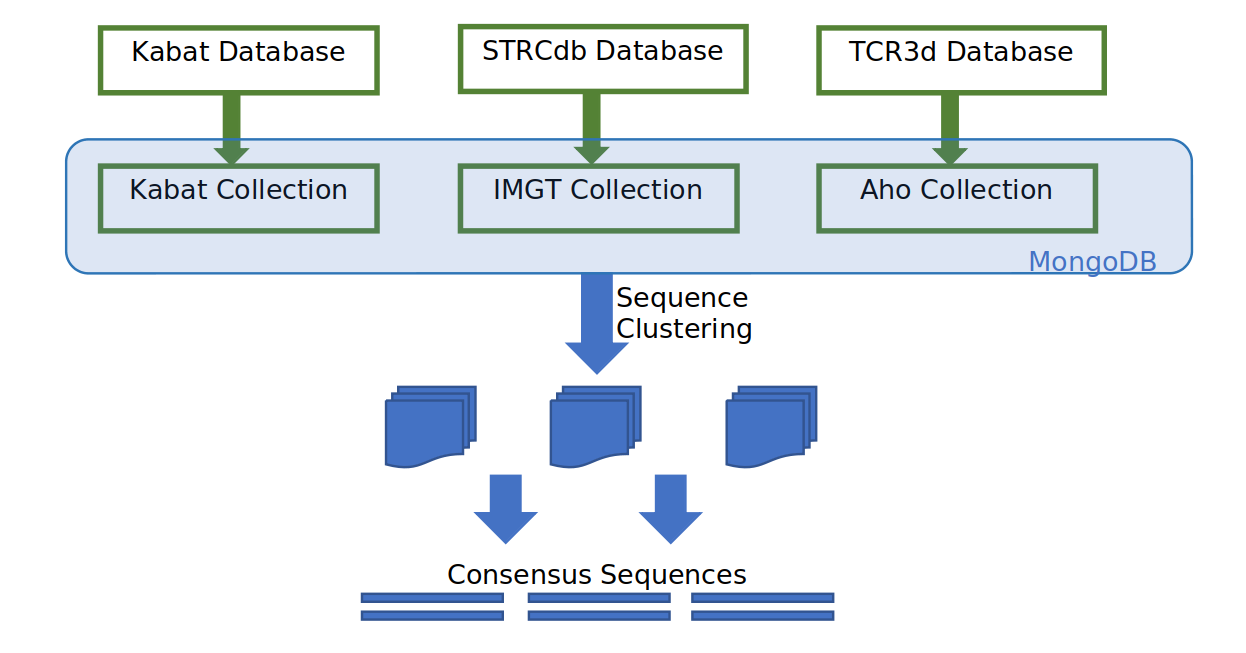
\includegraphics[width=\textwidth,height=\textheight,keepaspectratio]{database_creation.png}
    \caption{Consensus Sequence Creation. First, a MongoDB database is created, with three collections. These contain the parsed sequences with their meta data of Kabat, IMGT and Aho pre-numbered sequence databases. The sequences are then clustered (categorized by chain type). Residue frequency is analysed among the clusters to yield multiple consensus sequences, as well as conserved sequences.}
    \label{fig:database_creation}
\end{figure}


\begin{figure}
    \centering
    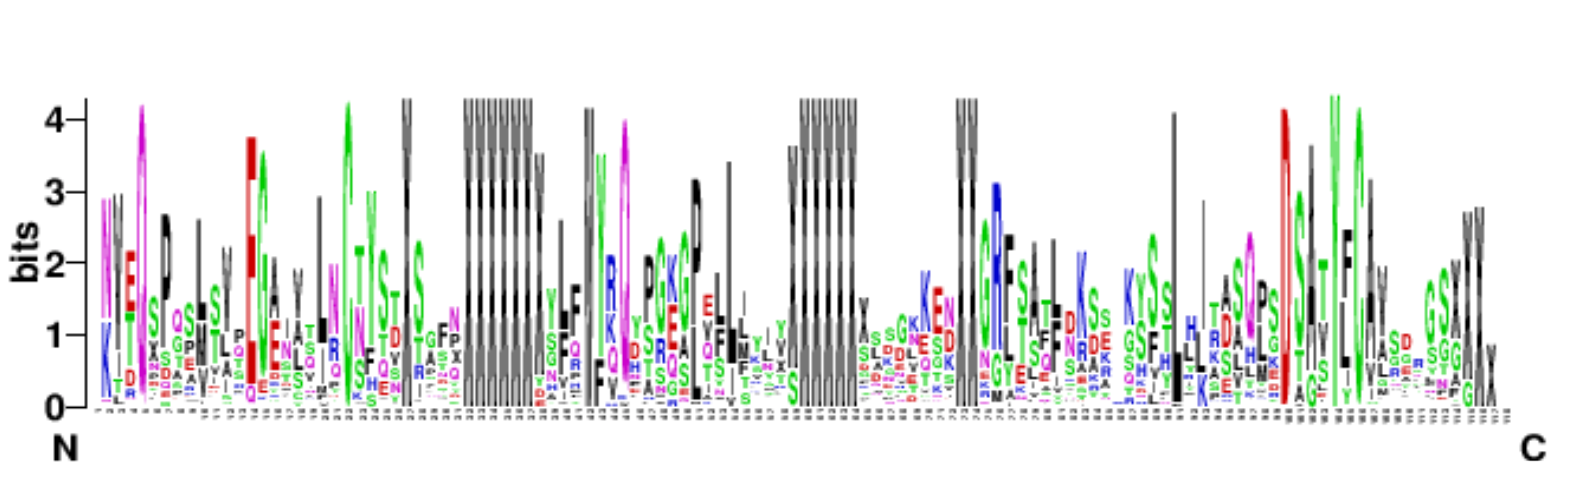
\includegraphics[width=\textwidth,height=\textheight,keepaspectratio]{Aho_logo.png}
    \caption{ Sequence Logo of TCR sequences in tcr3d database (Aho-numbered). Few conserved residues can be seen, as well as areas of greater sequence variability. Although some interesting features may be seen within this logo, there are many partial sequences in the  tcr3d database,which may distort some regions. }
    \label{fig:Aho_logo}
\end{figure}

\begin{figure}
    \centering
    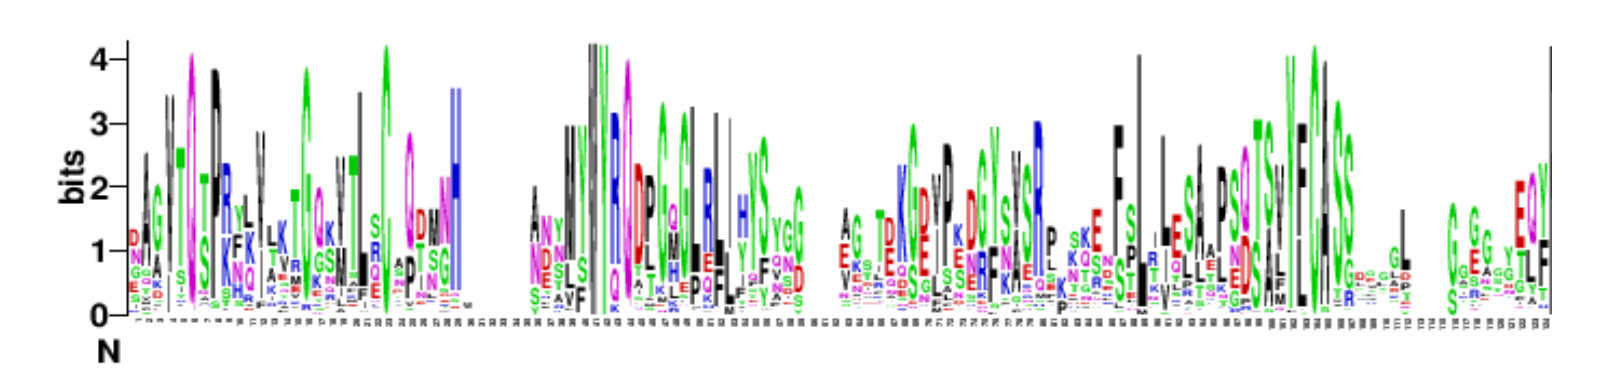
\includegraphics[width=\textwidth,height=\textheight,keepaspectratio]{IMGT_logo.png}
    \caption{Sequence Logo of TCR sequences in STRCdb database (IMGT-numbered). Few conserved residues can be seen, as well as areas of greater sequence variability. A similarity with Figure 2 can be seen. (Note:  the two figures have not been aligned according to sequence).}
    \label{fig:IMGT_logo}
\end{figure}

A consensus sequence can also be obtained for these sequences. Through prior sequence clustering by sequence identity, more informative consensus sequences can be produced\ref{fig:database_creation} The best-matching consensus sequence will then be selected for each sequence that is to be numbered in further steps. 

\subsection{Anchor Sequence Alignment}
In this equivalent to the AbNum-algorithm, sequence propensity profiles which are aligned to the sequence to find the CDR boundaries are used. By aligning short anchor sequences (10 \AA) built from sequence propensity profiles before and after CDR regions, the numbering can be filled in. The amino acid numbers are filled in from both sides in turn.

The sequence propensity profiles were built for each of the framework regions and CDRs using all organisms and chain types. Then, profiles were build for FR and CDRs separated by chain type, then separated by organism and lastly by both organism and chain type. 

[Most reliably, a large set of profiles separated by both organism and chain type will be used. The best match is selected for the first anchor alignment. The chain type and organism selection is then verified by matching other anchors of the same group to the sequence.]

Furthermore, the template was moved back by 5 residues in CDR3, due to a maximum deletion of 5AA in the V-region, to improve sequence profile alignment accuracy.


For the Kabat sequencing scheme, the profiles were built using exclusively sequences from the Kabat database. The profiles were used to number the entire cleaned Kabat dataset. For sequences that were incorrectly numbered, these were removed and new sequence profiles were built iteratively.
The manually removed sequences (after manually checking these were correctly numbered) were then used to create separate sequence profiles. 

As a fall-back a full length consensus sequence is used. The best consensus is determined by iterating through a set of consensus sequences, which are yielded from sequence clusters. 

\subsection{Modified Needleman-Wusch Algorithm}
This is a dynamic approach that implements a modification of the Needleman-Wunsch algorithm. 
Similar to AbRSA\cite{Li2019}, an algorithm for robust antibody numbering, a differentiation between CDR, 
FR and insertion positions within the scoring system is introduced. This yields a more refined alignment. 
Parameter optimization was employed for best results.

Multiple consensus sequences are obtained each for TCR chains α,β,γ,δ. The best-fitting consensus sequence for the input sequence is chosen, matching the input chain-type. Using the different CDR-definitions and insertion positions according to the numbering schemes, the consensus sequence residues are categorized as belonging to 1) framework region, 2) CDR, 3) insertion positions, 4) conserved positions. A score is calculated according to



\noindent With cells in the array numbered from 1:
\begin{equation*}
s[i,j] = (S(a[x,i],a[y,j]) *q) + \max\left\{ \begin{array}{l}
       s[i-1, j-1]\\
       s[i-1, J = (j-2)\ldots 1] - g\\
       s[I = (i-2)\ldots 1, j-1] - g
       \end{array} \right.
\end{equation*}
\noindent where:
\begin{equation*}
  \begin{array}{ll}
    S[a,b] &= \text{BLOSUM62 scoring matrix score for amino acids } a \text{ and } b\\
    a[x,i] &= \text{the amino acid at position } i \text{ in sequence } x \\
    g      &= \left\{ \begin{array}{l}
        P_{CPs}  \ if j \in conserved positions\\
        P_{IPs} \  if j \in insertion positions\\
        P_{FRs} \  if j \in Framework positions\\
        P_{CDRs} \  if j \in CDR positions\\
       \end{array} \right. \\
       
     q      &= \left\{ \begin{array}{l}
        S_{CPs}  \ if j \in conserved positions\\
        1 \  if j \in others\\
        \end{array} \right. \\
        
    n      &= (j-1) - J \text{ -or- } (i-1) - I\\
  \end{array}
\end{equation*}

\clearpage

The  values of P\textsubscript{CPs},  P\textsubscript{IPs} , P\textsubscript{FRs} and P\textsubscript{CDRs} are gap penalties. The value of S\textsubscript{CPs} is a weight for a matched conserved residue. The values are defined in the AbRSA paper \cite{Li2019}.

\subsection{HMM alignment}
In this approach Hidden Markov Model profiles are first generated for short sequences of 5 amino acids prior to and after a CDR-boundary. By aligning these to the sequence correctly, the start and end of these regions can be determined. After the CDR positions are correctly determined and verified, the numbering can be filled in according to the respective numbering scheme. 

\section{Methods}

\subsection{Database Creation}
For Kabat sequencing, the Kabat TCR database was downloaded. The sequences are separated by chain and organism. There is no need for sequence alignment using this database, as the input is pre-aligned. The sequences are then uploaded into a database (MongoDB). This is done to build a comprehensive database of manually annotated TCR sequences of all different numbering schemes investigated, which was not currently available. IMGT-annotated sequences are taken from the StCRDab\cite{Leem2018} database, which contains PDB files of human and mouse TCRs (αβ and γδ), Aho-numbered sequences were taken from the tcr3d database5\cite{Gowthaman2019} 

\subsection{Clustering Methods}
\subsubsection{CD-HIT}
Sequence clustering with CD-HIT\cite{Li2006} (70\% sequence identity)

\subsection{Consensus Sequence}
 Consensus sequences built by selecting residues with a position specific score (PSS) of above 50\%. Conserved residues are classified as those with a PSS \> 95\%.
 

\section{Discussion}

Upon evaluation of all tested numbering methods, the most robust approach was determined to be anchor sequence alignment. The numbering, when tested on the cleaned Kabat dataset, yielded accurate numbering in all but 12 cases. Of the failed instances, 4 of these sequences were sourced from "other" organisms. The source of the sequences could not yet be determined. 
The short-coming of the AbRSA-based method may be explained by insufficient optimization for the values of the gap penalty values and conserved position weights. 
A rudimentary version of the anchor-based method will be made available for sequence numbering at  \url{http://www.bioinf.org.uk/abs/qualiloop/TCRnum}. 


